\documentclass{article}

\usepackage{graphicx}
\usepackage{tikz}
\usepackage{tikzsymbols}
\usetikzlibrary{calc,patterns,shapes.geometric}
\pagestyle{empty}
\usepackage[margin=0pt]{geometry}
\geometry{papersize={14in,12in}}

\def\centerarc[#1](#2)(#3:#4:#5){\draw[#1] ($(#2)+({#5*cos(#3)},{#5*sin(#3)})$) arc (#3:#4:#5);}

\begin{document}
	\begin{figure}
		\centering
		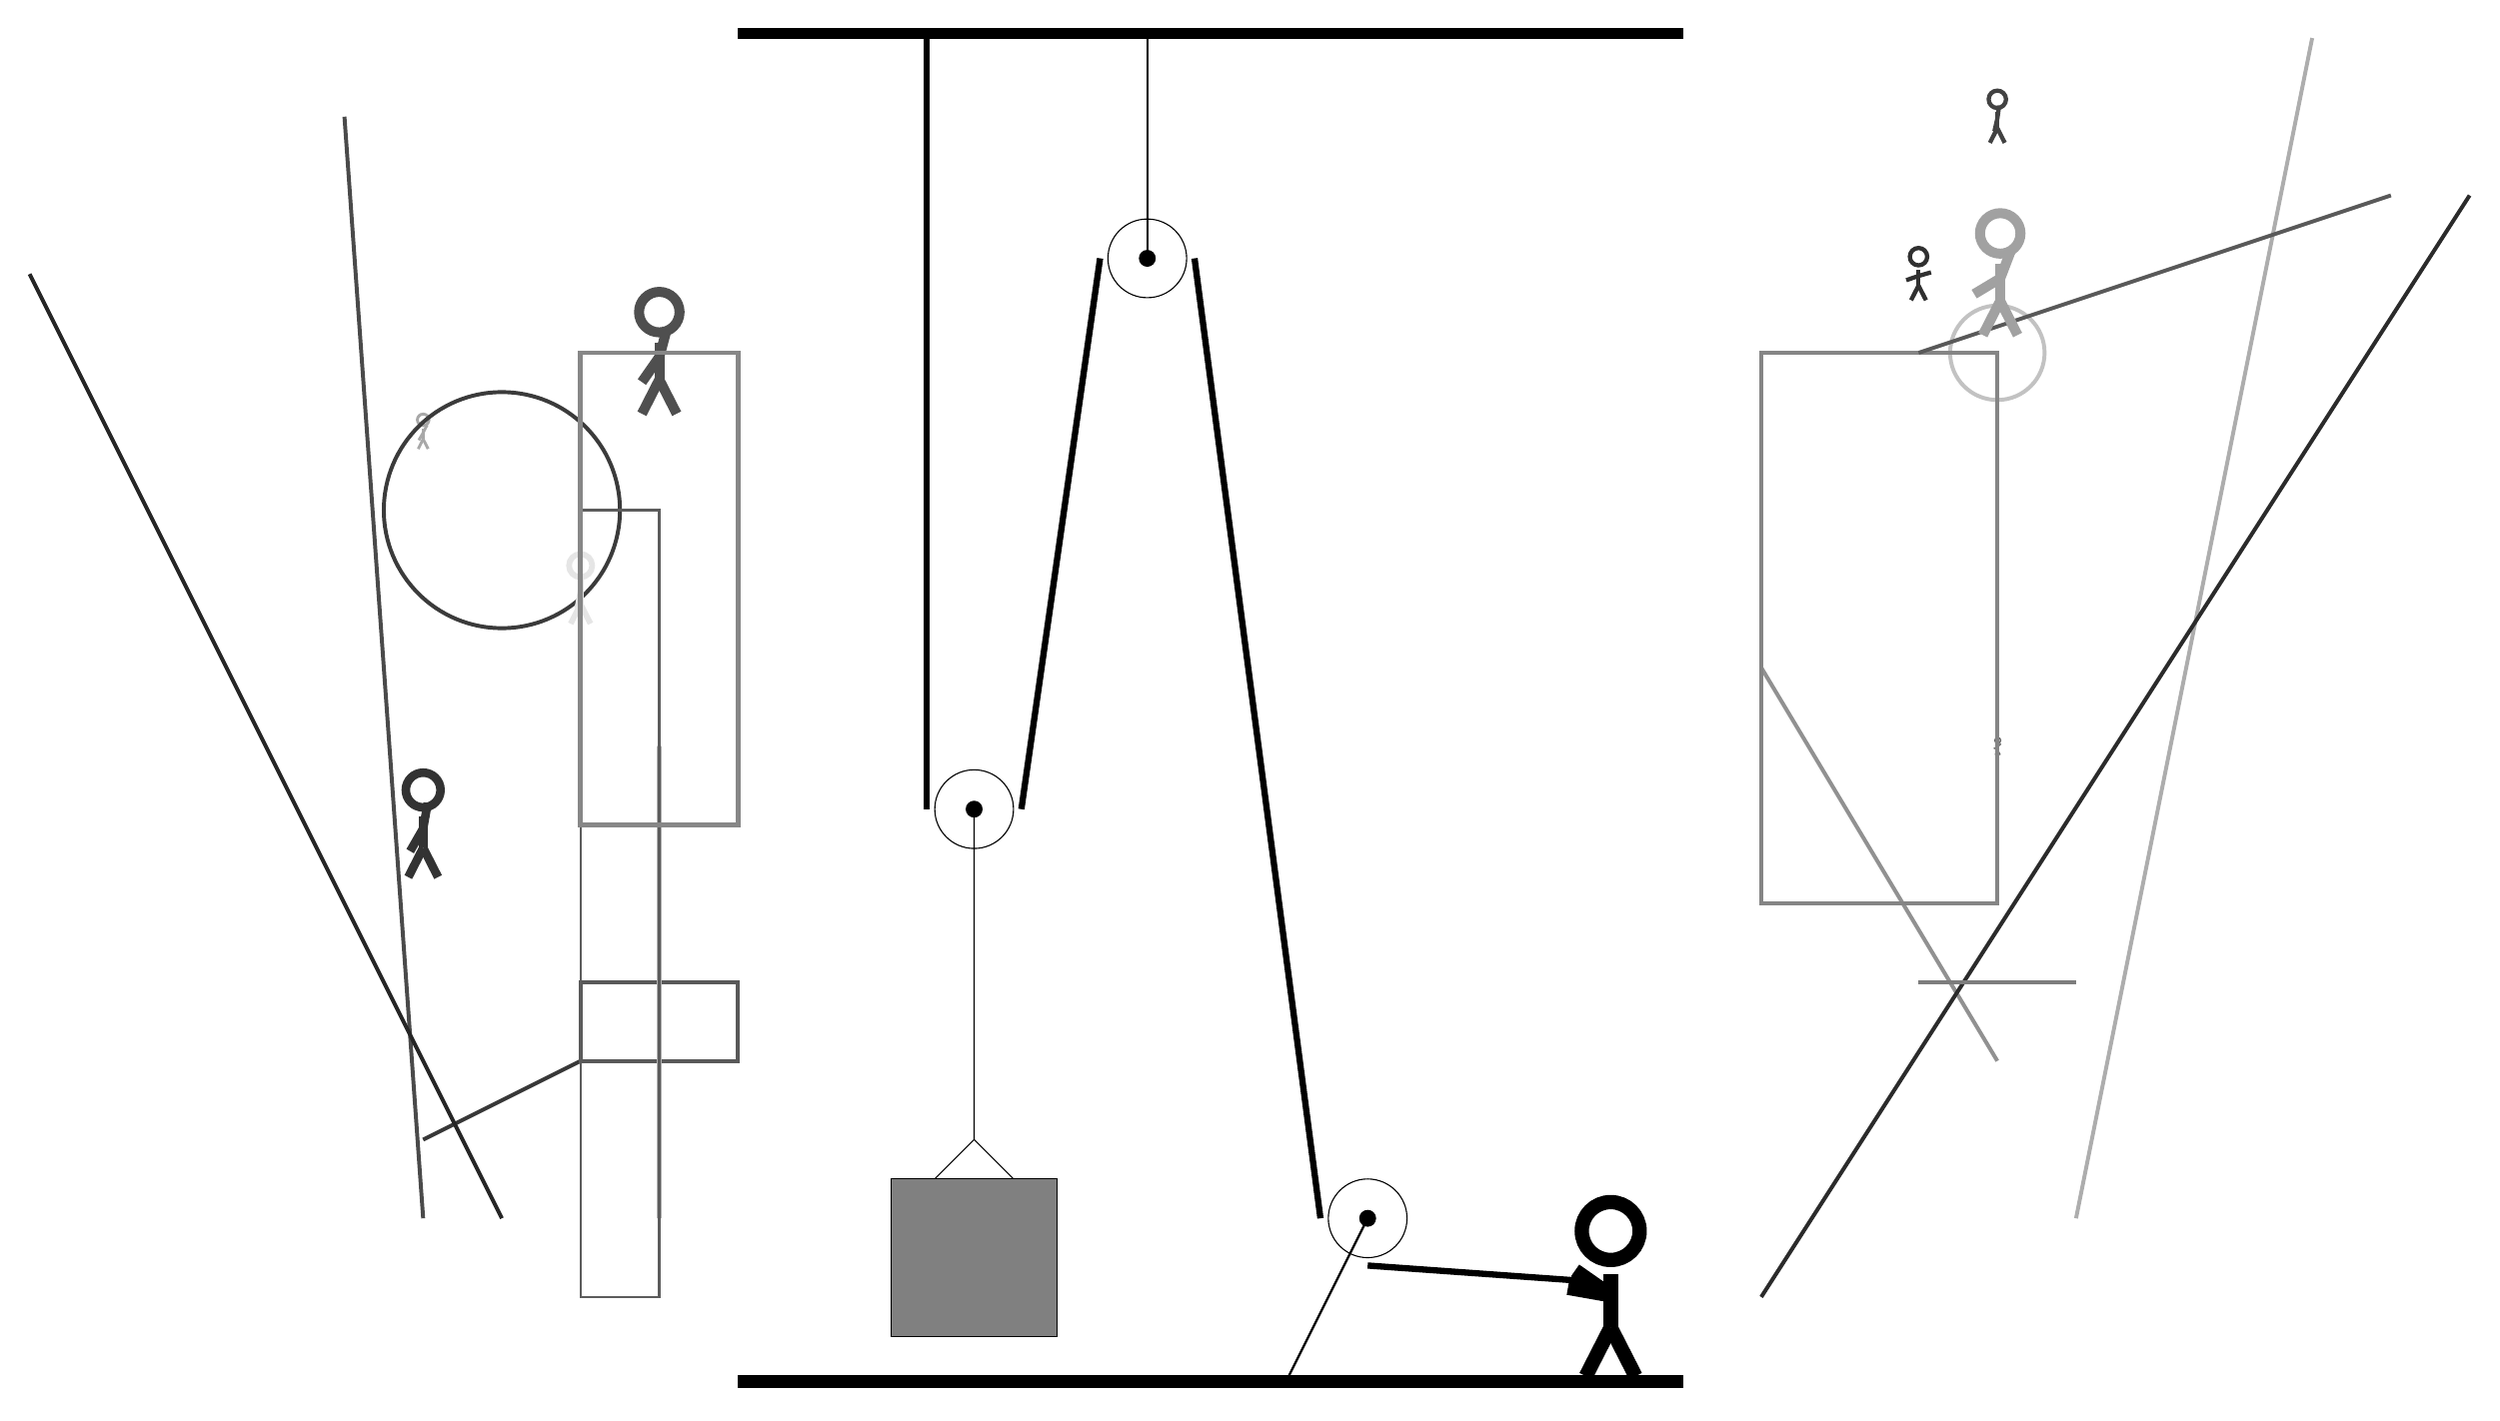
\begin{tikzpicture}
			%%%%% START %%%%%
			
			\draw[fill=black] (-2, 14) rectangle (10, 14.125);
			
			\draw (3.2, 11.2) circle (0.5);
			\draw[fill=black] (3.2, 11.2) circle (0.1);
			\draw[thick] (3.2, 11.2) -- (3.2, 14);
			
			\draw (6, -1) circle (0.5);
			\draw[fill=black] (6, -1) circle (0.1);
			\draw[thick] (6, -1) -- (5, -3);
			
			\draw (1, 4.2) circle (0.5);
			\draw[fill=black] (1, 4.2) circle (0.1);
			
			\draw (1, 4.2) -- (1, 0) -- (0.5, -0.5);
			\draw (1, 0) -- (1.5, -0.5);
			\draw[fill=black!50] (-0.05, -0.5) rectangle (2.05, -2.5);
			
			\draw[line width=0.5mm, color=black!78](-6, 0) -- (-4, 1);
			
			\node[line width=0.2mm, color=black!60] at (14, 5) {\Strichmaxerl[1][25][44]};
			\draw[line width=0.5mm, color=black!71](-7, 13) -- (-6, -1);
			\draw[line width=0.5mm, color=black!43](11, 6) -- (14, 1);
			
			\draw[line width=0.5mm, color=black!85](-5, -1) -- (-11, 11);
			\node[line width=0.6mm, color=black!34] at (-6, 9) {\Strichmaxerl[2][60][63]};
			\draw [line width=0.5mm, color=black!24](14, 10) circle (0.6);
			\node[line width=0.5mm, color=black!69] at (-3, 10) {\Strichmaxerl[7][55][75]};
			\node[line width=0.6mm, color=black!81] at (13, 11) {\Strichmaxerl[3][19][16]};
			\draw[line width=0.5mm, color=black!32](15, -1) -- (18, 14);
			\draw [line width=0.5mm, color=black!77](-5, 8) circle (1.5);
			\draw[line width=0.5mm, color=black!65] (-2, 2) rectangle (-4, 1);
			\draw[line width=0.5mm, color=black!48] (11, 10) rectangle (14, 3);
			\draw[line width=0.5mm, color=black!65](13, 10) -- (19, 12);
			\node[line width=0.3mm, color=black!80] at (-6, 4) {\Strichmaxerl[6][60][80]};
			\node[line width=0.2mm, color=black!74] at (14, 13) {\Strichmaxerl[3][77][82]};
			
			\draw[line width=0.7mm, color=black!31] (-3, 5) rectangle (-3, -1);
			\node[line width=0.4mm, color=black!10] at (-4, 7) {\Strichmaxerl[4][79][88]};
			\draw[line width=0.3mm, color=black!64] (-3, 8) rectangle (-4, -2);
			
			\draw[line width=0.5mm, color=black!83](11, -2) -- (20, 12);
			\node[line width=0.6mm, color=black!37] at (14, 11) {\Strichmaxerl[7][31][69]};
			
			\draw[line width=0.5mm, color=black!51](13, 2) -- (15, 2);
			\draw[line width=0.6mm, color=black!47] (-2, 4) rectangle (-4, 10);
			
			\draw[line width=0.8mm] (0.4, 14) -- (0.4, 4.2);
			\centerarc[line width=0.8mm](1, 4.2)(180:360:0.6);
			\draw[line width=0.8mm](1.6, 4.2) -- (2.6, 11.2);
			\centerarc[line width=0.8mm](3.2, 11.2)(0:180:0.6);
			\draw[line width=0.8mm](3.8, 11.2) -- (5.4, -1);
			\centerarc[line width=0.8mm](6, -1)(180:270:0.6);
			\draw[line width=0.8mm](6, -1.6) -- (8.8, -1.8);
			
			\node at (9, -1.9) {\Strichmaxerl[10][-35][170]};
			
			\draw[fill=black] (-2, -3) rectangle (10, -3.15);
			
			%%%%% END %%%%%
		\end{tikzpicture}
	\end{figure}	
\end{document}